%\documentclass[spanish]{beamer}
\documentclass{beamer}
\usepackage{pgf,pgfpages}
%\pgfpagesuselayout{4 on 1}[letterpaper,landscape,border shrink=0.5in]
\usepackage{algorithm,algorithmic}
%\usepackage{algorithm,algorithmicx}
%\usepackage[noend]{algpseudocode}
\usepackage{listings}
\lstset{basicstyle=\ttfamily,
	showstringspaces=false,
	commentstyle=\color{red},
	literate={á}{{\'a}}1
	{ã}{{\~a}}1
	{é}{{\'e}}1
	{É}{{\'E}}1
	{ó}{{\'o}}1
	{í}{{\'i}}1
	{ñ}{{\~n}}1
	{¡}{{!`}}1
	{¿}{{?`}}1
	{ú}{{\'u}}1
	{Í}{{\'I}}1
	{Ó}{{\'O}}1
}

\usepackage{beamerthemesplit}
\usepackage{color}
\usepackage[utf8]{inputenc}
\usepackage[spanish]{babel}
%\usepackage[latin1]{inputenc}
%\usepackage[pdftex]{graphicx}
%\usepackage{algorithm}
%\usepackage{algorithmic-C}
%\usepackage{algorithmic}
\usepackage{amsthm}
\usepackage{multicol}
\usepackage{multirow}
\usepackage{fancyvrb,relsize}
\usepackage{hhline}
\usepackage{tikz}
\usetikzlibrary{trees, shapes, calc}
\newcommand{\inputTikZ}[2]{%
	\scalebox{#1}{\input{#2}}
}

\usetheme{Warsaw} %Gueno
%\usetheme{Darmstadt} %OK!
% \usetheme{Frankfurt} %OK!
%\usetheme{Goettingen}
%\usetheme{Dresden}
%\usetheme{JuanLesPins} %OK!!
%\usetheme{Marburg}
%\usetheme{Montpellier}
%\usetheme{Rochester} %sobrio
%\usetheme{Singapore}
%\usetheme{Szeged}

%\usecolortheme{albatross}
%\usecolortheme{seahorse}
%\usecolortheme{beetle}
%\usecolortheme{crane}
%\usecolortheme{dolphin}
%\usecolortheme{dove}
%\usecolortheme{fly}
%\usecolortheme{lily} %Gueno
\usecolortheme{orchid}%Gueno
%\usecolortheme{rose}
%\usecolortheme{seagull}
%\usecolortheme{whale}


\DefineVerbatimEnvironment%
      {VerbatimNN}%
      {Verbatim}%
      {fontsize=\relsize{-1}}
\DefineVerbatimEnvironment%
      {VerbatimNNN}%
      {Verbatim}%
      {fontsize=\relsize{-2}}

\DefineVerbatimEnvironment%
      {VerbatimPseudo}%
      {Verbatim}%
      {numbers=left, fontsize=\relsize{-1}}
\DefineVerbatimEnvironment%
      {VerbatimPseudoReduced}%
      {Verbatim}%
      {numbers=left, fontsize=\relsize{-2}}
\DefineVerbatimEnvironment%
      {VerbatimPseudoReduced2}%
      {Verbatim}%
      {numbers=left, fontsize=\relsize{-3}}
\DefineVerbatimEnvironment%
      {VerbatimC}%
      {Verbatim}%
      {commandchars=@ªº, numbers=left, fontsize=\relsize{-1}}
\DefineVerbatimEnvironment%
      {VerbatimReducedC}%
      {Verbatim}%
      {commandchars=@ªº, numbers=left, fontsize=\relsize{-2}}
\DefineVerbatimEnvironment%
      {VerbatimReduced2C}%
      {Verbatim}%
      {commandchars=@ªº, numbers=left, fontsize=\relsize{-3}}



%\AtBeginSubsection[]
%{
% \begin{frame}
% \frametitle{Sinopsis}
% Aqui decides: cada seccion y subseccion:
% \tableofcontents[currentsection,currentsubsection]
 %O solamente la seccion (Solo uno de ellos)
%\tableofcontents[currentsection]
% \end{frame}
%}

% Si quieres que todo por default aparezca de poco en poco
% descomenta esta linea
%\beamerdefaultoverlayspecification{<+->}

\setbeamertemplate{footline}{\hfill\insertframenumber/\inserttotalframenumber}
\setbeamertemplate{navigation symbols}{}

\setbeamercovered{transparent}

\title{ELO320 - Estructuras de Datos y Algoritmos\\Análisis de Complejidad: F. Recurrencia\\\small{Método Maestro}}
%\subtitle{Ingeniería Civil Telemática UTFSM}
\author{Dr. Nicolás Gálvez R.\\{\small nicolas.galvez@usm.cl}}
\institute{Ing. Civil Telemática - Departamento de Electrónica}
\titlegraphic{
\includegraphics[scale=.18]{images/logoutfsm}}
\date{1er Semestre 2025}

\begin{document}

\frame{\titlepage}

%\section*{Sinopsis}
%\frame{  \frametitle{Sinopsis}\tableofcontents[pausesections]}
%
%

\section{Recuento: Funciones de Recurrencia}
\begin{frame}[fragile]
 \frametitle{Funciones de Recurrencia}
\small
¿Cómo podemos determinar la complejidad de MergeSort si éste trabaja recursivamente?
\begin{itemize}
\item Peor escenario: $\mathcal{O}(n \log n)$
\item Mejor escenario: $\Omega(n \log n)$
\item Escenario Promedio: $\Theta(n \log n)$
\end{itemize}

\textbf{Funciones de recurrencia}, relaciones matemáticas recursivas que son utilizadas en ciencias de la computación para explicar la complejidad de éste tipo de algoritmos.
\end{frame}

\begin{frame}[fragile]
 \frametitle{Funciones de Recurrencia}
\small
\begin{exampleblock}{Factorial}
\begin{lstlisting}[language=C, basicstyle=\tiny, escapeinside={|}{|}]
int factorial(int n){
	if(n>0)
		exit(-1);

	if(n==0)
		return 1;
	return n * factorial(n-1); // 1 + T(n-1)
}
\end{lstlisting}
\end{exampleblock}

Sabemos:
\begin{itemize}
\item $T(n) = 1$ (si $n = 0$).
\item $T(n) = 1 + T(n-1)$ (si $n > 0$).
\item Luego: $T(n) = 1 + 1 + 1 + \dots + T(1) = n$.\pause
\item $T(n) = n \rightarrow \mathcal{O}(n)$.
\end{itemize}
\end{frame}


\begin{frame}[fragile]
 \frametitle{Funciones de Recurrencia}
\small
\begin{exampleblock}{Búsqueda Binaria}
\begin{lstlisting}[language=C, basicstyle=\tiny, escapeinside={|}{|}]
int binarySearch(int arr[], int l, int r, int x){
    if (r >= l) {
        int mid = l + (r - l) / 2;

        if (arr[mid] == x) 
            return mid;

        if (arr[mid] > x) //if-else 1 + T(n/2)
            return binarySearch(arr, l, mid - 1, x);
	return binarySearch(arr, mid + 1, r, x); //else
    }

    return -1;
}
\end{lstlisting}
\end{exampleblock}


\begin{itemize}
\item $T(n) = 1$ (si $n = 1$). $T(n) = 1+ T(n/2) $ (si $n > 1$).
\item Luego: $T(n) = 1 + 1 + 1 + \dots + T(n/2^k)$ \pause
\item Al finalizar: $T(n/2^k) = T(1) \rightarrow n = 2^k$ \pause
\item $\log_2 n  = log_2(2^k) \rightarrow k = \log_2 n $ \pause 
\item $ T(n) = 1 + T(n/2) = 1 + \mathcal{O}(\log n) = \mathcal{O}(\log n)$
\end{itemize}
\end{frame}


\begin{frame}[fragile]
 \frametitle{Funciones de Recurrencia}
\small
\begin{exampleblock}{MergeSort}
\begin{lstlisting}[language=C, basicstyle=\tiny, escapeinside={|}{|}]
void mergeSort(int arr[], int l, int r){ //l=izq, r=der (indices)
    if (l < r) {
        int m = l + (r - l) / 2; // |$\mathcal{O}(1)$|

        mergeSort(arr, l, m); // T(n/2)
        mergeSort(arr, m + 1, r); // T(n/2)

        merge(arr, l, m, r); // |$\mathcal{O}(n)$| 
    }
}
\end{lstlisting}
\end{exampleblock}


\begin{itemize}
\item $T(n) = 1$ (si $n = 1$).
\item $T(n) = n + 2 \times T(n/2) $ (si $n > 1$).
\item $T(n) = n (1 + \log n) = n + n \log n$
\item $T(n) = \mathcal{O}(n \log n) $
\end{itemize}
\end{frame}

\section{Método Maestro}
\begin{frame}[fragile]
 \frametitle{Método Maestro}
\small
Desarrolle el árbol de recurrencia para la siguiente función:
$$ T(n) = T(n/2) + T(n/4) + n^2 $$

\begin{itemize}
\item ¿Cuál es la rama más larga? ¿Qué significa?
\item ¿Cuál es la rama más corta? ¿Qué significa?
\end{itemize}
\end{frame}

\begin{frame}[fragile]
 \frametitle{Método Maestro}
\small Técnica para cálculo inmediato de complejidades promedio ($\Theta$) bajo ciertas condiciones basado en el árbol de recurrencia de dichas funciones.

\begin{block}{Método Maestro}
Sea: 
$$ T(n) = a \times T\Big(\frac{n}{b}\Big) + f(n) $$
Con $a \geq 1$, $b > 1$, $f(n) > 0 $ para $n \geq n_0$ con $n_0 \geq 0$. 
\end{block}

\begin{itemize}
\item Largo/Altura: $\log_{b} n$
\item Cantidad hojas: $a^{\log_{b} n} = n^{\log_{b} a}$
\item Costos: $T(n) = \sum_{j=0}^{log_{b}(n-1)} a^j f(\frac{n}{b^j}) + \Theta(n^{log_{b}a})$
\end{itemize}
\end{frame}



\begin{frame}[fragile]
 \frametitle{Método Maestro}
\small Técnica para cálculo inmediato de complejidades promedio ($\Theta$) bajo ciertas condiciones basado en el árbol de recurrencia de dichas funciones.

\begin{block}{Método Maestro}
Sea: 
$$ T(n) = a \times T\Big(\frac{n}{b}\Big) + f(n) $$
Con $a \geq 1$, $b > 1$, $f(n) > 0 $ para $n \geq n_0$ con $n_0 \geq 0$. 
\begin{itemize}
\item Caso 1:\\
\smallskip
Si $f(n) = \mathcal{O}(n^{\log_b a - \epsilon})$ con $\epsilon > 0 \pause \rightarrow T(n) = \Theta(n^{\log_b a})$.
\end{itemize}
\end{block}
Note que acá buscamos que $\log_b a$ sea mayor que el grado de complejidad $c$ ($\mathcal{O}(n^c)$). 
\end{frame}

\begin{frame}[fragile]
 \frametitle{Método Maestro}
\small Técnica para cálculo inmediato de complejidades promedio ($\Theta$) bajo ciertas condiciones basado en el árbol de recurrencia de dichas funciones.

\begin{exampleblock}{Método Maestro}
Sea: 
$$ T(n) = a \times T\Big(\frac{n}{b}\Big) + f(n) $$
Con $a \geq 1$, $b > 1$, $f(n) > 0 $ para $n \geq n_0$ con $n_0 \geq 0$. 
\begin{itemize}
\item Caso 2:\\
\smallskip
Si $f(n) = \Theta(n^{\log_b a} \log^k n)$ con $k \geq 0 \pause \rightarrow T(n) = \Theta(n^{\log_b a} \log^{k+1} n)$.
\end{itemize}
\end{exampleblock}
Note que acá buscamos que $\log_b a$ sea igual que el grado de complejidad $c$ ($\Theta(n^c)$). 
\end{frame}

\begin{frame}[fragile]
 \frametitle{Método Maestro}
\small Técnica para cálculo inmediato de complejidades promedio ($\Theta$) bajo ciertas condiciones basado en el árbol de recurrencia de dichas funciones.

\begin{alertblock}{Método Maestro}
Sea: 
$$ T(n) = a \times T\Big(\frac{n}{b}\Big) + f(n) $$
Con $a \geq 1$, $b > 1$, $f(n) > 0 $ para $n \geq n_0$ con $n_0 \geq 0$. 
\begin{itemize}
\item Caso 3:\\
\smallskip
Si $f(n) = \Omega(n^{\log_b a + \epsilon})$ con $\epsilon > 0$ y\\
$a f(\frac{n}{b}) \leq c f(n)$ con $c < 1$ y $n \rightarrow \infty$.\\\pause
Luego: 
$\rightarrow T(n) = \Theta(f(n))$
\end{itemize}
\end{alertblock}
Note que acá buscamos que $\log_b a$ sea menor que el grado de complejidad $c$ ($\Omega(n^c)$).
\end{frame}

\begin{frame}[fragile]
 \frametitle{Método Maestro}
El método maestro busca determinar quien elemento predomina en la complejidad del algoritmo que usa recursividad:
\begin{itemize}
\item Caso 1: Trabajo de las hojas es polinomialmente mayor, y por ende, domina la complejidad $n^{\log_b a}$.
\item Caso 2: Trabajo entre hojas y raíz es asintóticamente igual, entonces complejidad es \texttt{nodo} $\times$ \texttt{altura}, vale decir, $f(n) \times \log_n$.
\item Caso 3: Trabajo en la raíz es polinomialmente mayor, y por ende, domina la complejidad $f(n)$.
\end{itemize}
\end{frame}


\begin{frame}[fragile]
 \frametitle{Funciones de Recurrencia: Ejemplos}
\small
Desarrolle las siguientes funciones de recurrencia, y determine su desempeño promedio $\Theta$ usando el método maestro:
\begin{itemize}
\item $T(n) = 9T(n/3) + n$
\item $T(n) = 4T(n/2) + n^2 $
\item $T(n) = 5T(n/5) + n^3 $
\item $T(n) = T(n/4) + T(n/2) + n^2$ ¿Se puede?
\item $T(n) = 2T(n/2) + n$
\item $T(n) = 49T(n/7) + 1$ 
\item $T(n) = 2T(n/2) + \frac{n^2}{\log n}$ ¿Es posible?
\end{itemize}
\end{frame}


%\begin{frame}[fragile]
% \frametitle{Análisis Asintótico: Big O ($\mathcal{O}$)}
%\small Cota asintótica que limita el peor desempeño de un algoritmo.
%
%\begin{exampleblock}{Big O ($\mathcal{O}$)}\small
%Sean $f$ y $g$ dos funciones en $\mathbb{R}$, diremos que:
%$$f(n) = \mathcal{O}(g(n)) \iff f(n) \in \mathcal{O}(g(n))$$
%Donde:
%$$ \mathcal{O}(g(n)) = \{f(n)\ |\ \exists c \in \mathbb{R}, f(n) \leq c \times g(n);\ \forall n \geq n_0\}$$
%\end{exampleblock}
%
%\begin{center}
%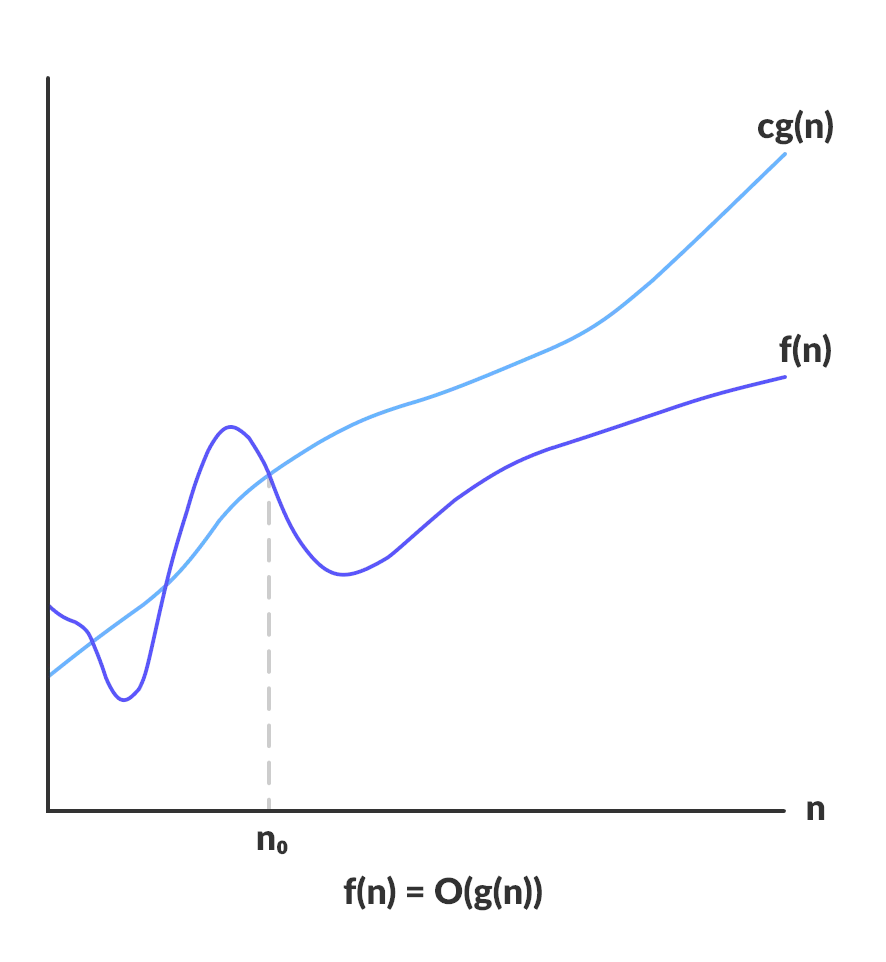
\includegraphics[width=.35\linewidth]{images/bigO}
%\end{center}
%
%\end{frame}
%
%\begin{frame}[fragile]
% \frametitle{Análisis Asintótico: Big Omega ($\Omega$)}
%\small Cota asintótica que limita el mejor desempeño de un algoritmo.
%
%\begin{exampleblock}{Big Omega ($\Omega$)}\small
%Sean $f$ y $g$ dos funciones en $\mathbb{R}$, diremos que:
%$$f(n) = \Omega(g(n)) \iff f(n) \in \Omega(g(n))$$
%Donde:
%$$ \Omega(g(n)) = \{f(n)\ |\ \exists c \in \mathbb{R},  c \times g(n) \leq f(n) ;\ \forall n \geq n_0\}$$
%\end{exampleblock}
%
%\begin{center}
%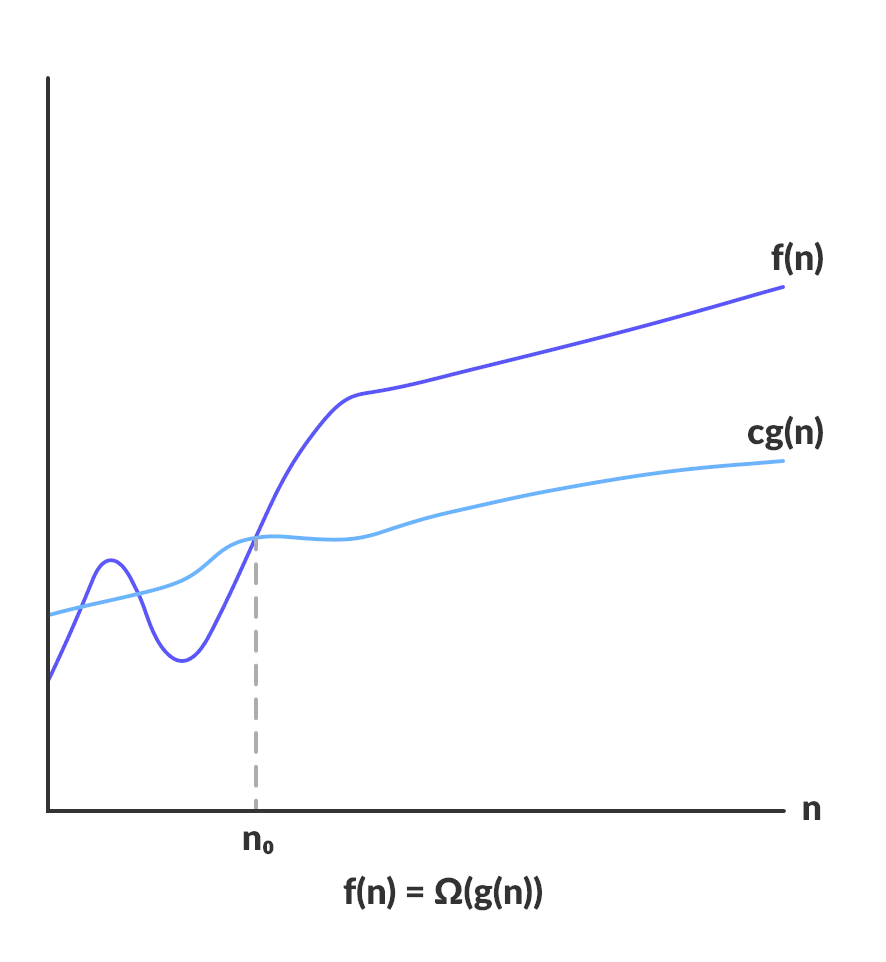
\includegraphics[width=.35\linewidth]{images/bigOmega}
%\end{center}
%
%\end{frame}
%
%\begin{frame}[fragile]
% \frametitle{Análisis Asintótico: Big Theta ($\Theta$)}
%\small Cota asintótica que limita el desempeño promedio de un algoritmo.
%
%\begin{exampleblock}{Big Theta ($\Theta$)}\small
%Sean $f$ y $g$ dos funciones en $\mathbb{R}$, diremos que:
%$$f(n) = \Theta(g(n)) \iff f(n) \in \Theta(g(n))$$
%Donde:
%$$ \Theta(g(n)) = \{f(n)\ |\ \exists (c_1, c_2) \in \mathbb{R}^2, c_1 \times g(n) \leq f(n) \leq c_2 \times g(n);\ \forall n \geq n_0\}$$
%\end{exampleblock}
%
%\begin{center}
%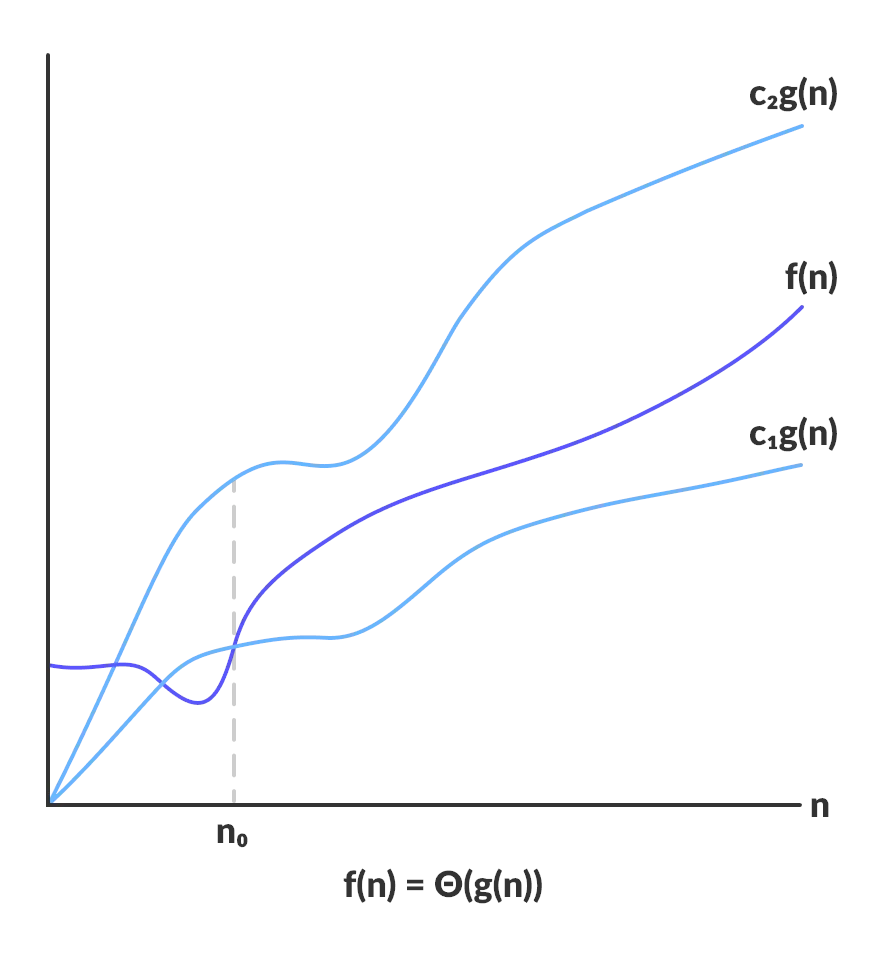
\includegraphics[width=.35\linewidth]{images/bigTheta}
%\end{center}
%
%\end{frame}
%
%\begin{frame}[fragile]
% \frametitle{Análisis Asintótico}
%\begin{exampleblock}{¿Cuál es la complejidad del siguiente algoritmo}
%\begin{lstlisting}[language=C, basicstyle=\tiny, escapeinside={|}{|}]
%int suma(int n) {
%	int sum = 0, i, j;
%	for (i=0; i < n; i++) 
%		for (j=0; j < n; j++)
%			sum++;
%	return sum;
%}
%\end{lstlisting}
%\end{exampleblock}
%\small
%\pause
%\begin{itemize}
%\item Costo total $f(n) =$ \pause $6n^2 + 10n + 8 $.
%\item $g(n) = n^2$, termino del grado superior.
%\item Cota superior: \texttt{suma} $= \mathcal{O}(n^2)$ \pause $\rightarrow$ \pause $f(n) \leq 7 \times g(n) $
%\item Cota inferior: \texttt{suma} $= \Omega(n^2)$ \pause $\rightarrow$ \pause $5 \times g(n) \leq f(n) $
%\item Cota promedio: \texttt{suma} $= \Theta(n^2)$ \pause $\rightarrow$ \pause $5 \times g(n) \leq f(n) \leq 7 \times g(n)$
%\end{itemize}
%\end{frame}
%
%\begin{frame}[fragile]
% \frametitle{Análisis Asintótico}
%\small
%\begin{center}
%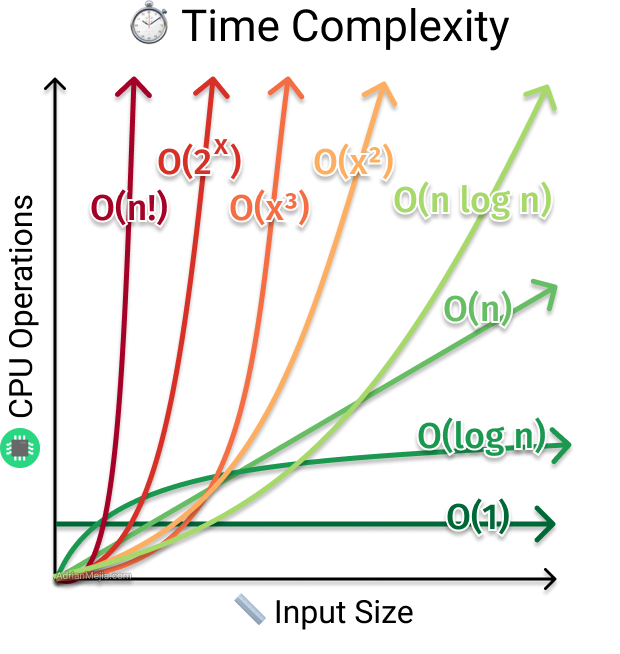
\includegraphics[width=.7\linewidth]{images/timecomplexity2}
%\end{center}
%\end{frame}
%
%
%\begin{frame}[fragile]
% \frametitle{Análisis Asintótico}
%\small
%\begin{center}
%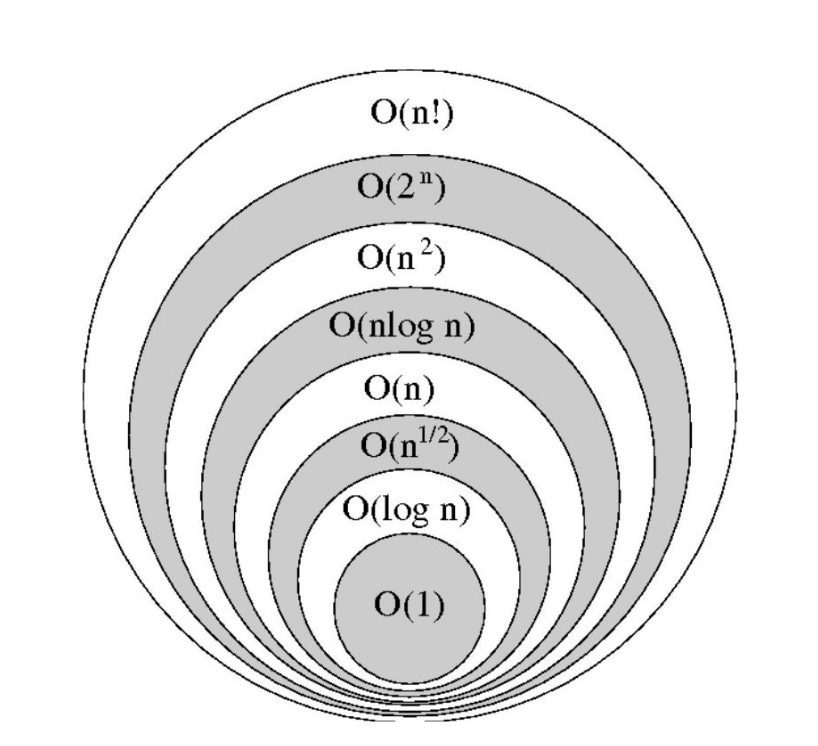
\includegraphics[width=.7\linewidth]{images/bigO2}
%\end{center}
%\end{frame}
%
%\section{Insertion Sort}
%\begin{frame}[fragile]
% \frametitle{InsertSort}
%\small Es un método de ordenamiento de elementos, en el cual a través de la visitas de subconjuntos, un elemento es \textbf{insertado} en la posición ordenada que le corresponde.
%
%\begin{center}
%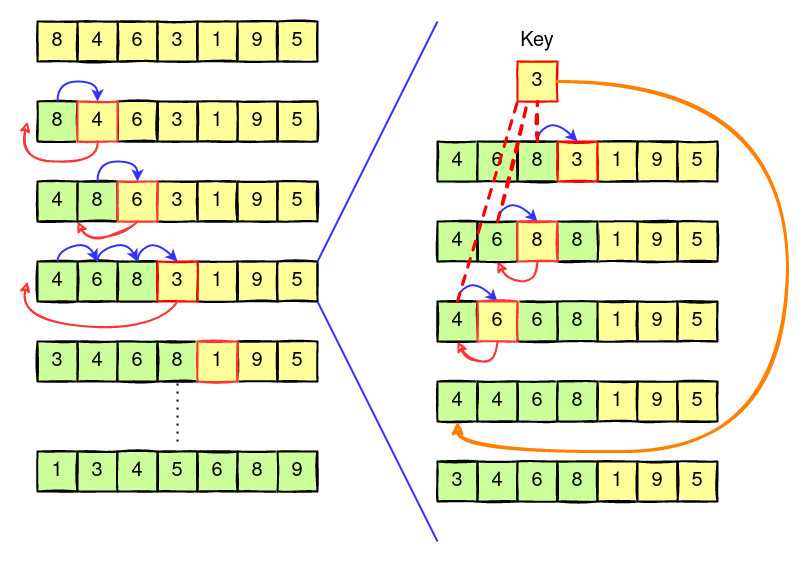
\includegraphics[width=.7\linewidth]{images/InsertSort}
%\end{center}
%\end{frame}
%
%\begin{frame}[fragile]
% \frametitle{InsertSort}
%\begin{exampleblock}{¿Cuál es la complejidad del siguiente algoritmo}
%\begin{lstlisting}[language=C, basicstyle=\tiny, escapeinside={|}{|}]
%void insertionSort(int arr[], int n){
%	int i, key, j;
%	for (i = 1; i < n; i++) {
%		key = arr[i];
%		j = i - 1;
% 		while (j >= 0 && arr[j] > key) { //esto puede ser un for
%			arr[j + 1] = arr[j];
%			j--;
%		}
%        	arr[j + 1] = key;
%    	}
%}
%\end{lstlisting}
%\end{exampleblock}
%\end{frame}
%
%\begin{frame}[fragile]
% \frametitle{InsertSort: Complejidad}
%
%\begin{itemize}
%\item Cota Superior: $\mathcal{O}(n^2) \rightarrow$ Caso peor: todo invertido. 
%\item Cota Inferior: $\Omega(n) \rightarrow$ Mejor caso: todo ordenado.
%\item Cota Promedio: $\Theta(n^2) \rightarrow$ Caso promedio para arreglos aleatorios. 
%\end{itemize}
%
%Extrapolando a otros algoritmos, ¿Por qué generalmente se usa $\mathcal{O}$ y no $\Theta$? Debido a que en muchos algoritmos, $\Theta$ no es sostenible para TODOS los casos.
%
%\end{frame}
%
%\begin{frame}[fragile]
% \frametitle{Ejercicios}
%\small
%\begin{itemize}
%\item Revisite las implementaciones de listas, pilas, colas y árboles y determine la complejidad de sus métodos.
%\item Mostrar la evolución de Insert Sort en el arreglo A = {31, 41, 59, 26, 41, 58}
%\item Reescribir Insert Sort para ordenamiento de datos de manera decreciente.
%\item Expresar la ecuación n3/1000 - 100n2 - 100n + 3 en términos de notación asintótica.
%\item Considere el problema de sumar dos números enteros expresados base binaria, almacenados en dos arreglos A y B de n elementos (bits) cada uno. La suma de los dos enteros se debe almacenar en forma binaria en un arreglo C de (n+1) elementos. Escriba una función en C para la suma los dos enteros. ¿Qué complejidad tiene su función? Compárela con la de sus compañeros.
%\end{itemize}
%\end{frame}


\end{document}
